\section{Stegvis-deduktiv induktiv metode}
\label{section:sdi} 
Analyse av kvalitative data betegner en prosess hvor forskerne forsøker å forstå de empiriske dataene som er samlet inn. Analysen av datamaterialet er blitt utført etter en SDI-metodisk tilnærming (se figur \ref{SDI}). \citet{Tjora} beskriver denne som \textit{$"$en skjematisk modell for kvalitativ forskning, hvor grunnprinsippet er en induktiv utvikling fra empiri til konsepter eller teorier, med deduktive trinnvise tilbakekoblinger. Målet er konseptutvikling og kvalitetssikring.$"$} De oppadgående pilene viser den induktive prosessen hvor forskningen er empiridrevet, mens de nedadgående pilene viser det deduktive arbeidet hvor forskningen i større grad er teoridrevet.

\begin{figure}[H]
\centering
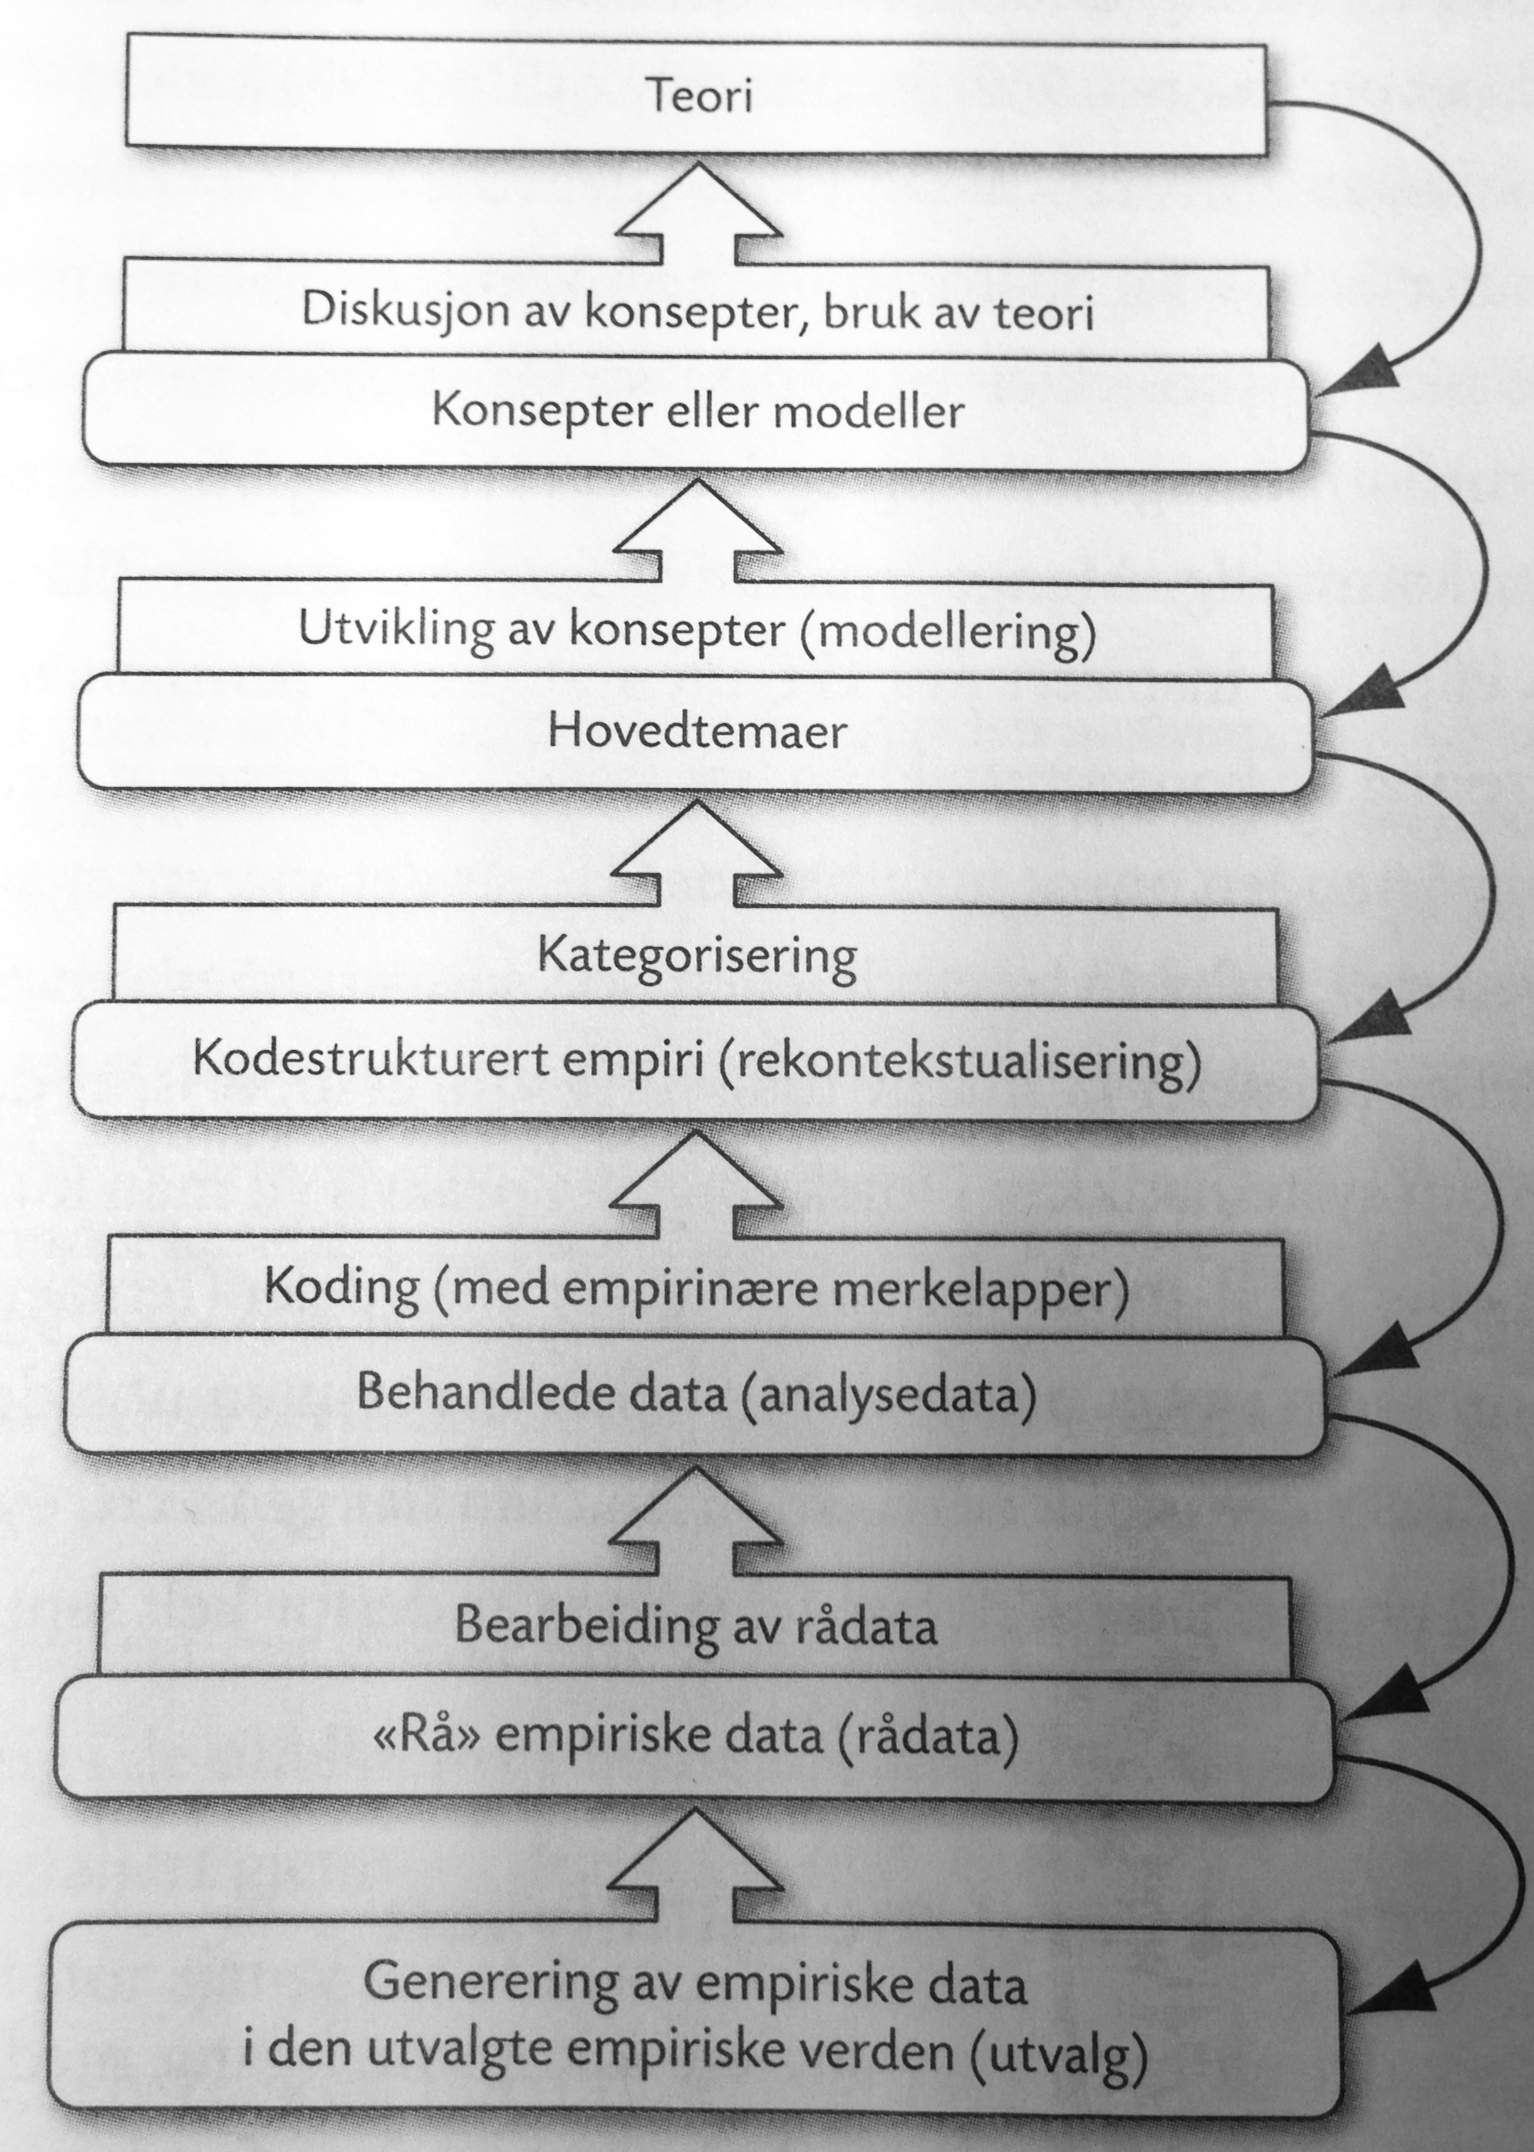
\includegraphics[scale=1]{SDI.jpg}
\caption{Stegvis-deduktiv induktiv metode \citep{Tjora})}
\label{SDI}
\end{figure}

\noindent
Feltnotatene fra første observasjonsperiode ble transkribert, og deretter kodet og kategorisert ved bruk av dataprogrammet RStudio \citep{Rstudio}. Kodingen av observasjonsdataene resulterte i nærmere 100 koder, og forskerne jobbet på denne måten induktivt med materialet. Det høye antallet koder forklares ved at forskerne genererte detaljerte, tekstnære koder fra en stor mengde data \citep{Tjora}. For å kunne luke ut empiri som ikke var relevant for videre forskning ble kodene kategorisert i 11 kategorier. Dette ga en strukturert oversikt over forskningsområdet og forskerne formulerte forskningsspørsmål som det videre arbeidet søkte svar på. Arbeidet beveget seg dermed fra konseptutviklingsfasen til en ny runde med generering av empiriske data. Feltnotatene fra andre observasjonsperiode ble kodet og kategorisert med nærmere 50 koder og 5 kategorier. Etter observasjonsperioden utpekte det seg dermed sentrale temaer som videre formet intervjuguidene. Lydopptakene fra intervjuene ble transkribert og brukt som støtte til observasjonsdataene for å utdype, sammenligne og avdekke forskjeller mellom forskernes og informantenes oppfatninger. Avslutningsvis forsøkte forskerne å konseptualisere avdekkede funn ved å diskutere disse i lys av relevant teori. 


